\chapter{Programm}
\label{chap:Programm}

\section{Parameter des Fluggeräts}
\label{sec:parameter_fluggeraet}
Bei der Auslegung des Fluggeräts werden nicht nur Multicopter betrachtet sondern auch Flächenflugzeuge, sogenannte fixed wing UAVs. Aus diesem Grund werden die Parameter Motor, Propeller, Batterie und Missionsparameter sowie Umgebungsparameter allgemein für beide Arten der UAVs festgelegt. Anschließend werden die Parameter des Multicopters oder des Flächenflugzeugs bestimmt, je nachdem, welches Fluggerät untersucht werden soll. 
Das Programm und die diesem grundlegende Leistungsberechnung, basieren auf dem internen Bericht "Leistungsberechnung von Multicoptern" von Y. Beyer (2016). Aus dieser wurden die Berechnung der Aerodynamik von Multicoptern, die Pulsweitenmodulation und der Batterieentladung sowie die festgelegten Grenzen der fliegbaren Flugzustände übernommen. 
 
\subsubsection{Flugsystem}
Zu Beginn der Mission muss das Flugsystem festgelegt werden, da jeweils nur eins zu jedem Zeitpunkt untersucht werden kann. Die Abfrage erfolgt mit der Variablen \texttt{Abfrage\_Flugsystem}. Diese kann die Werte \texttt{1} für einen Multicopter oder \texttt{0} für ein Flächenflugzeug annehmen.

\subsubsection{Motor}
Die ersten drei Motorparameter sind notwendig, um den Motorzustand zu berechnen. Der letzte Parameter dient als technische Grenze, die für ein gut ausgelegtes System nicht überschritten wird. Die Motormasse fließt in Kombination mit der Anzahl der Propeller in die Gesamtmasse des Fluggerätes mit ein.

\begin{center}
	\captionof{table}{Motorparameter für technische Grenzen}
	\begin{tabular}{l l l} \hline
		 Parameter & Variablenname & Einheit \\ \hline
		 Innenwiderstand \ensuremath{R_i} & \texttt{R\_i} & \SI{}{\ohm} \\
		 Geschwindigkeitskonstante \ensuremath{K_v} & \texttt{K\_V} & \ensuremath{\frac{RPM}{V}} bzw. \ensuremath{\frac{U}{Vs}} \\
		 Leerlaufstrom \ensuremath{I_0} & \texttt{I\_O} & \ensuremath{A}  \\
		 maximaler Dauerstrom \ensuremath{I_{max}} & \texttt{I\_max} & \ensuremath{A} \\
		 Motormasse \ensuremath{m_{Mot}} & \texttt{m\_Mot} & \ensuremath{kg} \\ \hline
	\end{tabular}	
	\label{tab:mot_parameter}
\end{center}

\subsubsection{Propeller}
Der Propellername wird in der Form 'Durchmesser x Pitch' angegeben. Der Name ist wichtig, um das Propellerkennfeld aus Propellerdatenbank von APC zu entnehmen. Die Anzahl der Propeller beeinflusst entscheidend die Geometrie des Fluggerätes. Weiterhin wird damit der benötigte Schub auf die Anzahl der Propeller aufgeteilt. Die letzten Parameter dienen zur Bestimmung Anströmung und der Berücksichtigung der Blattelemententheorie.

\begin{center}
	\captionof{table}{Propellerparameter für Schub, aerodynamische und technische Grenzen}
	\begin{tabular}{l l l} \hline
		 Parameter & Variablenname & Einheit \\ \hline
		 Propellername & \texttt{prop\_name} & \ensuremath{-} \\
		 Anzahl der Propeller \ensuremath{n_{Prop}} & \texttt{n\_Prop} & \ensuremath{-} \\
		 Mittlerer Nullwiderstandsbeiwert \ensuremath{c_{d0}} & \texttt{c\_d0} & \ensuremath{0,05} \\
		 Anstieg des Auftriebsbeiwerts \ensuremath{\frac{dc_a}{dc_\alpha}} & \texttt{a\_alpha} & \ensuremath{5} \\
		 Maximaler Anstellwinkel \ensuremath{\alpha_{max}} & \texttt{alpha\_stall} & \ensuremath{10}\textdegree \\ \hline
	\end{tabular}	
	\label{tab:prop_parameter}
\end{center}

\subsubsection{Batterie}
Die aufgeführten Parameter der Batterie bestimmen zum einen die verfügbare Kapazität und zum anderen die Batterieentladung. Bei der Energiedichte handelt es sich um repräsentative Werte für den verwendeten Akkutyp, z.B. Li-Ion oder Li-Po. Die minimale Zellenspannung ist ein Erfahrungswert, der am \textit{Institut für Flugführung} verwendet wird. Um den Energieverlust der Batterie zu berechnen, wird die Peukert-Konstante herangezogen. Diese beträgt für Li-Po-Akkus ca. $1,01 \leq P \leq 1,05$ und für Li-Ion-Akkus ca. 1,05 (\textcolor{red}{Traub}). Außerdem sind Lithium Batterien stark temperaturempfindlich. Niedrige Temperaturen als die Umgebungstemperatur können die angegebene Nennkapazität reduzieren und die Verluste progressiv steigen lassen. Die maximale C-Rate dient als weitere technische Begrenzung, die wiederum für ein gut ausgelegtes System nicht erreicht wird.

\begin{center}
	\captionof{table}{Batterieparameter zur Berechnung der verbleibenden Restladung sowie der technischen Grenzen}
	\begin{tabular}{l l l} \hline
		 Parameter & Variablenname & Einheit \\ \hline
		 Energiedichte \ensuremath{\frac{E_{Bat}}{m_{Bat}}}& \texttt{E\_Dichte} & \ensuremath{J/kg} \\
		 Anzahl der Batteriezellen \ensuremath{N_{Bat,cell}} & \texttt{N\_bat\_cell} & \ensuremath{-} \\
		 nominale Spannung pro Batteriezelle \ensuremath{U_{Bat,cell}} & \texttt{U\_bat\_nom} & \ensuremath{V} \\
		 minimale Spannung pro Batteriezelle \ensuremath{U_{Bat,cell,min}} & \texttt{U\_bat\_min} & \ensuremath{V} \\
		 Peukert-Konstante \ensuremath{P}& \texttt{P\_bat\_Peukert} & \ensuremath{1,05} \\
		 Maximale C-Rate \ensuremath{C_{rate,max}} & \texttt{C\_Rate\_max} & \ensuremath{-} \\
		 Batteriemasse \ensuremath{m_{Bat}} & \texttt{m\_bat} & \ensuremath{kg} \\ \hline
	\end{tabular}	
	\label{tab:bat_parameter}
\end{center}

\subsubsection{Multicopter}
Die Parameter für den Multicopter sind in \ref{tab:multicop_parameter} aufgeführt. Die Leermasse fließt mit in die Gesamtmasse mit ein und wird für die Berechnung des Schubs und weiterer Parameter benötigt. Die Beiwerte sind reine Schätzwerte. Für die nachfolgenden Berechnungen ist nur die obere Stirnfläche von Bedeutung, da sich auf diese die Beiwerte beziehen. Die Propeller bleiben bei den Stirnflächen unberücksichtigt.
\begin{center}
	\captionof{table}{Parameter des Multicopters}
	\begin{tabular}{l l l} \hline
		 Parameter & Variablenname & Einheit \\ \hline
		 Leermasse des Multicopters \ensuremath{m_{Copter}} & \texttt{m\_copter} & \ensuremath{kg}\\
		 Obere Stirnfläche \ensuremath{A_{copter,oben}} & \texttt{A\_copter} & \ensuremath{m^2}\\
		 seitliche Stirnfläche \ensuremath{A_{copter,seitlich}} & \texttt{A\_copter\_seitlich} & \ensuremath{m^2}\\
		 Oberer Widerstandsbeiwert \ensuremath{c_{W,copter,oben}} & \texttt{c\_W\_copter\_oben} & \ensuremath{-}\\
		 Seitlicher Widerstandsbeiwert \ensuremath{c_{W,copter,seitlich}} & \texttt{c\_W\_copter\_seitlich} & \ensuremath{-}\\
		 Maximaler Auftriebsbeiwert \ensuremath{c_{A,copter,max}} & \texttt{c\_A\_copter\_max} & \ensuremath{-}\\ \hline
	\end{tabular}	
	\label{tab:multicop_parameter}
\end{center}

\subsubsection{Flächenflugzeug}
Der erste Parameter des Flächenflugzeugs wird zur Ermittlung des Bahnanstellwinkels benötigt. Für den Steigflug wird ein Flug mit optimaler Gleitzahl \ensuremath{E} vorausgesetzt. Mit der Leermasse wird analog zum Multicopter der Schub berechnet.
\begin{center}
	\captionof{table}{Parameter des Flächenflugzeug}
	\begin{tabular}{l l l} \hline
		 Parameter & Variablenname & Einheit \\ \hline
		 Reziproke Gleitzahl \ensuremath{\varepsilon} & \texttt{epsilon} & \ensuremath{-}\\		 
		 Leermasse des Flächenflugzeug \ensuremath{m_{Flugzeug}}& \texttt{m\_flugzeug} & \ensuremath{kg}\\ \hline
	\end{tabular}	
	\label{tab:flugzeug_parameter}
\end{center}

\section{Parameter der Mission}
\label{sec:parameter_mission}

\subsubsection{Missionsparameter}
Innerhalb der Flugparameter kann die Nutzlast \texttt{m\_Nutz} des Fluggerätes bestimmt werden. Diese Masse fließt mit der Masse des Motors und der der Motoren sowie der der Batterie in die Gesamtmasse mit ein. Im Rahmen des Projektes AEROMET UAV ist diese auf \SI{250}{g} festgelegt.
 
\subsubsection{Flugparameter}
Die Flugparameter geben für den Multicopter den Steigwinkel sowie die Steigeschwindigkeit vor.
\begin{center}
	\captionof{table}{Flugparameter}
	\begin{tabular}{l l l} \hline
		 Parameter & Variablenname & Einheit \\ \hline
		 Bahngeschwindigkeit \ensuremath{V_{Kg}} & \texttt{V\_Kg} & \ensuremath{m/s}\\		 
		 Bahnneigungswinkel \ensuremath{\gamma}& \texttt{gamma} & \ensuremath{^\circ}\\ \hline
	\end{tabular}	
	\label{tab:flugparameter}
\end{center}

\subsubsection{Umgebungsparameter}
Die Erdbeschleunigung und der Adiabatenexponent werden als konstant über der Höhe angenommen. Mit Startwerten für die Höhe, die Temperatur, die Dichte und des Luftdrucks werden die Abflugbedingungen am Abflugort spezifiziert.  Die Schrittweite der Höhe legt die Genauigkeit der Höhendiskretisierung fest.
\begin{center}
	\captionof{table}{Umgebungsparameter}
	\begin{tabular}{l l l} \hline
		 Parameter & Variablenname & Einheit \\ \hline
		 Erdbeschleunigung \ensuremath{g} & \texttt{g} & 9,81 \ensuremath{m/s^2} \\
		 Starthöhe \ensuremath{H_0} & \texttt{H\_0} & \ensuremath{m} \\
		 Schrittweite der Höhe  \ensuremath{\Delta H} & \texttt{Delta\_H} & \ensuremath{m} \\
		 maximale Höhe \ensuremath{H_{max}} & \texttt{H\_max} & \ensuremath{m} \\
		 Umgebungstemperatur am Start \ensuremath{T_0} & \texttt{T\_0} & \ensuremath{K} \\
		 Luftdruck am Start \ensuremath{p_0} & \texttt{p\_0} & \ensuremath{N/m^2} \\
		 Dichte am Start \ensuremath{\rho_0} & \texttt{rho\_0} & \ensuremath{kg/m^3} \\
		 Adiabatenexponent \ensuremath{\kappa} & \texttt{kappa} & \SI{1,4}{} \\
		 Windgeschwindigkeit \ensuremath{u_{Wg}} & \texttt{u\_Wg} & \ensuremath{m/s} \\ \hline
	\end{tabular}	
	\label{tab:umgebungs_parameter}
\end{center}

\section{Berechnung weiterer Parameter}
\begin{center}
	\captionof{table}{Berechnung weiterer Parameter}
	\begin{tabular}{l l l} \hline
		 Parameter & Variablenname & Gleichung\\ \hline
		 Nominale Batteriespannung & \texttt{U\_Bat\_nom} & \ensuremath{U_{Bat,nom} = N_{Bat,cell}\cdot U_{Bat,cell}} \\
		 Minimale Batteriespannung & \texttt{U\_Bat\_min} & \ensuremath{U_{Bat,min} = N_{Bat,cell}\cdot U_{Bat,cell,min}} \\
		 Propellerradius & \texttt{R} & \ensuremath{R = D\cdot 0,0254/2} \\
		 Fläche eines Propellers & F & \ensuremath{F = \pi\cdot R^2} \\
		 Temperatur in \SI{11}{km} Höhe & \texttt{T\_11} & \ensuremath{T_{11} = T_0 - 0.0065\cdot(11000-H_0)} \\
		 Dichte in \SI{11}{km} Höhe & \texttt{rho\_11} & \ensuremath{\rho_{11} = \rho_0\cdot\Big(1 - 0.0065\cdot\frac{11000}{T_0}\Big)^{4.256}} \\
		 Druck in \SI{11}{km} Höhe & \texttt{p\_11} & \ensuremath{p_{11} = p_0\cdot\Big(1 - 0.0065\cdot\frac{11000}{T_0}\Big)^{5.256}} \\ \hline
	\end{tabular}	
	\label{tab:umgebungs_parameter}
\end{center}



\section{Parameter der Mission}
\newpage
\section{Aufbau des Programms}
\label{sec:aufbau_des_programms}
Der Aufbau des \textsc{Matlab}-Skriptes wird im Struktogramm (abb. blabla) verdeutlicht.
\begin{figure}[H]
\centering
	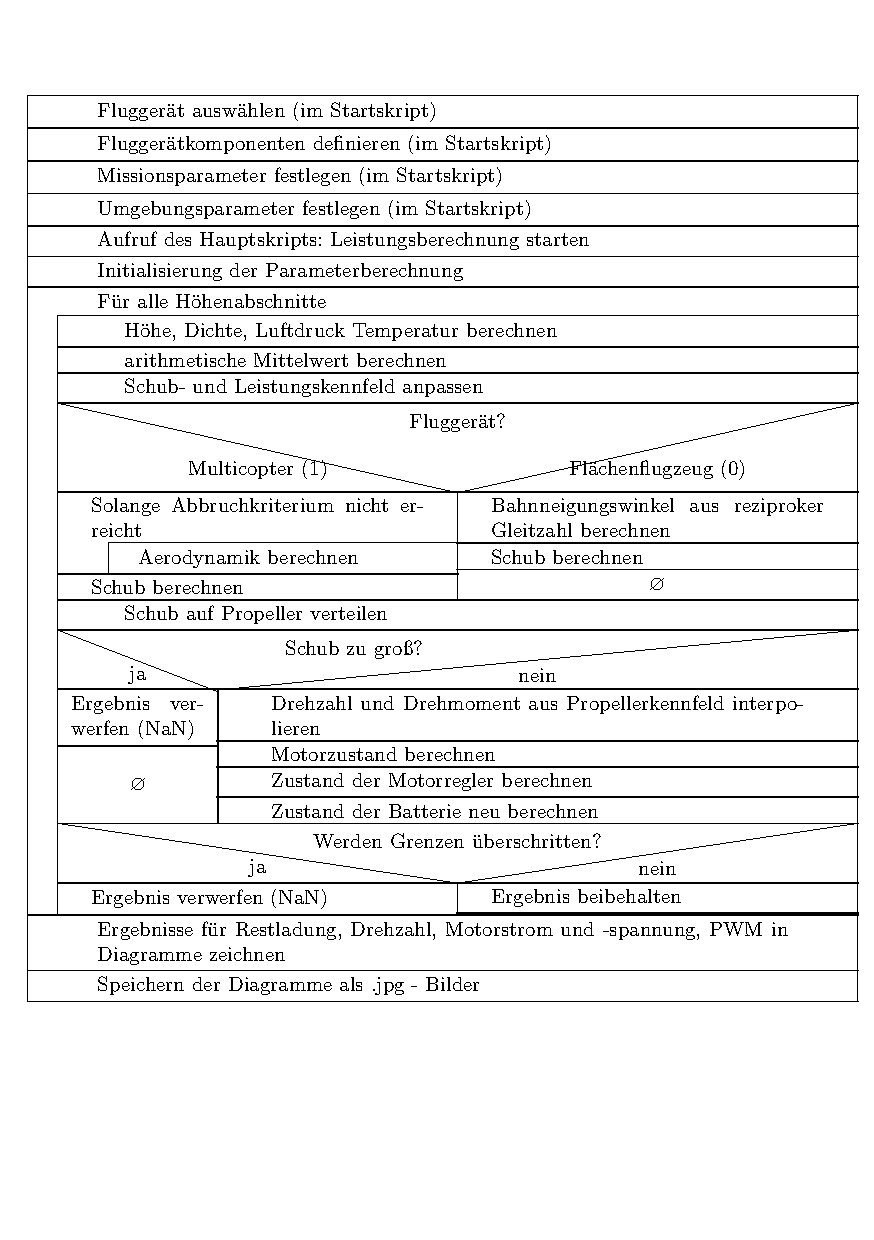
\includegraphics{Struktogramm/Struktogramm.pdf}
	\caption{Struktogramm des MATLAB-Skripts}
	\label{abb:struktogramm}
\end{figure}
\section{Leistungsberechnung}
\label{sec:leistungsberechnung}
\subsection{Veränderung der Umgebungsparameter mit der Höhe}
Für Leistungsuntersuchung wird die Internationale Standardatmosphäre vorausgesetzt. Hiernach ist der Temperaturkoeffizient bis zur Tropopause
\begin{equation}
	\frac{dT}{dH} = -0,0065\frac{K}{m}
\end{equation}
und danach in der unteren Stratosphäre bis zu einer Höhe von \SI{20000}{m}
\begin{equation}
	\frac{dT}{dH} = 0.
\end{equation}
Entsprechend kann der Verlauf der Temperatur, des Druckes und der Dichte mit
\begin{equation}
	T_{0-11} = T_0 - \frac{dT}{dH}\cdot H,
\end{equation}
\begin{equation}
	p_{0-11} = p_0\cdot [1-0,0065\frac{K}{m}\cdot \frac{H}{T_0}]^{5,256},
\end{equation}
\begin{equation}
	\rho_{0-11} = \rho_0 \cdot [1-\frac{dT}{dH}\cdot \frac{H}{T_0}]^{4,256}
\end{equation}
beschrieben werden. Ab \SI{20000}{m} ist der Verlauf von Druck und Dichte durch die Gleichungen
\begin{equation}
	p = p_{11}\cdot e^{\frac{g}{R\cdot T_{11}}\cdot (H-H_{11})},
\end{equation} 
\begin{equation}
	\rho = \rho_{11}\cdot e^{\frac{g}{R\cdot T_{11}}\cdot (H-H_{11})}
\end{equation}
gegeben.
Um den Einfluss der Flughöhe in der Leistungsberechnung festzuhalten, werden für jedes Höhenintervall die Umgebungsparameter an den oberen und unteren Intervallgrenzen berechnet. Durch Bildung des arithmetischen Mittelwertes ergeben sich daraus durchschnittliche Parameter für den Höhenabschnitt.  

\subsection{Schub berechnen}
\subsubsection{Multicopter}
Der Schub des Multicopters setzt sich zusammen aus dem zu kompensierenden Gewicht und dem Luftwiderstand durch eine Fluggeschwindigkeit. Dazu kommt noch indirekt der ebenfalls zu kompensierende Seitenwind. Innerhalb eines iterativen Modells wird die Aerodynamik berechnet. Hierbei sind der Auftriebs- und Widerstandsbeiwert Funktionen des modifizierten Anstellewinkels. Die Idee des Aerodynamischen Modells entstammt aus Beyer,Y.2016b. 
Die Gesamtmasse des Multicopters setzt sich aus der Masse des Rahmens mit anderen Einheiten wie z.B. dem ESC, der Masse der Batterie, der Masse der Motoren und der Nutzlast
\begin{equation}
	m = m_{copter}+m_{Bat}+m_{Mot}\cdot n_{Prop}+m_{Nutz}
\end{equation}
zusammen.
Die absolute Fluggeschwindigkeit setzt sich zusammen aus Seitenwindgeschwindigkeit und Bahngeschwindigkeit
\begin{equation}
	V_A = \sqrt{(u_{Kg} + u_{Wg})^2+w_{Kg}}
\end{equation}
mit
\begin{equation}
	\begin{pmatrix} u_{Kg} \\ w_{Kg} \end{pmatrix} = \begin{pmatrix}
	\cos\gamma \\ -sin{\gamma}	\end{pmatrix} \cdot V_{kg}.
\end{equation}
Die am Multicopter angreifenden Kräfte werden in Abbildung(einfügen) dargestellt. 
\begin{center}

\includegraphics[scale=0.5]{images/Coming-Soon.jpg}
\end{center}
Für die spätere Koordinatentransformation wird der Windanstellwinkel
\begin{equation}
	\gamma_a = \arctan \Big(\frac{-w_{Kg}}{u_{Kg}+u_{Wg}}\Big)
\end{equation}
berechnet.
Die Iteration beginnt mit \ensuremath{\Theta_0=0} und der Berechnung des modifizierten Anstellwinkels
\begin{equation}
	\alpha_M = \Theta '-\gamma_a.
\end{equation}
Im Anschluss werden die aerodynamischen Beiwerte 
\begin{equation}
	c_W = \frac{c_{W,copter,oben}-c_{W,copter,seitlich}}{2}\cdot \cos(2\cdot \alpha_M)+\frac{c_{W,copter,oben}+c_{W,copter,seitlich}}{2}
\end{equation} und 
\begin{equation}
	c_A = c_{A,max}\cdot sin(2\cdot \alpha_M)
\end{equation}
berechnet. Mit diesen folgt die Berechnung der aerodynamischen Kräfte
\begin{equation}
	W = c_W\cdot \frac{\rho}{2}\cdot A_{copter,oben}\cdot V_A^2,
\end{equation}
\begin{equation}
	A = c_A\cdot \frac{\rho}{2}\cdot A_{copter,oben}\cdot V_A^2.
\end{equation}
Die aerodynamischen Kräfte werden dann vom aerodynamischen Koordinatensystem in das geodätische Koordinatensystem transformiert:
\begin{equation}
	\begin{pmatrix} X^A \\ Y^A \\Z^A \end{pmatrix}_g = \begin{pmatrix} \cos\gamma_a & 0 & -\sin\gamma_a \\ 0 & 1 & 0 \\ \sin\gamma_a & 0 & \cos\gamma_a \end{pmatrix}^T\cdot \begin{pmatrix} -W \\ 0 \\ -A \end{pmatrix}_a = \begin{pmatrix} -W\cdot\cos\gamma_a-A\cdot\sin\gamma_a \\ 0 \\ W\cdot\sin\gamma_a-A\cdot\cos\gamma_a \end{pmatrix}_g.
\end{equation}
Der Neigungswinkel kann aus dem Kräftegleichgewicht
\begin{equation}
	\Theta_i' = -\arctan\Big(\frac{-X_g^A}{Z_g^A + m\cdot g}\Big), \qquad i =1,2,3,\dots
\end{equation}
neu berechnet werden und geht als Startwert in den nächsten Iterationsschritt ein. Die Iteration erfolgt solange bis das Abbruchkriterium
\begin{equation}
	\Delta\Theta' = \Theta_i-\Theta_{i-1}\stackrel{!}{<}0,001^{\circ}
\end{equation}
erreicht wird. 
Ist das Abbruchkriterium erreicht, kann der erforderliche Schub mit dem Satz des Pythagoras aus den Kraftanteilen in \(x_g-\) und \(z_g-\)Richtung
\begin{equation}
	S = \sqrt{{X_g}^2+(Z_g^A+m\cdot g)^2}
\end{equation}
bestimmt werden.
Für den Fall, dass der errechnete Schub größer als der zur Verfügung stehende Schub ist, wird das Ergebnis verworfen und als \texttt{NaN} (Not a Number) gespeichert.

\subsubsection{Flächenflugzeug}
Der Schub für ein Flächenflugzeug berechnet sich aus der Kompensation des Widerstandes und des Anteils der Gewichtskraft. Analog zum Multicopter setzt sich die Gesamtmasse des Flächenflugzeugs aus der Summe aller Komponenten zusammen
\begin{equation}
	m = m_{flugzeug}+m_{Bat}+m_{Mot}\cdot n_{Prop}+m_{Nutz}.
\end{equation}
Aus dem Kräftegleichgewicht aller angreifenden Kräfte am System können folgende Beziehungen 
\begin{equation}
	F = W + \sin\gamma\cdot G,
\end{equation}
\begin{equation}
	A = \cos\gamma G
\end{equation}
entnommen werden.
Mit
\begin{equation}
	E = \frac{A}{W}
\end{equation}
bzw.
\begin{equation}
	\varepsilon = \frac{W}{A} = \frac{c_W}{c_A}
\end{equation} 
können die Gleichungen umgeformt werden zu
\begin{equation}
	F = G\cdot\cos\gamma\cdot\Big(\frac{1}{E}+\tan\gamma\Big) = G\cdot(\sin\gamma+\varepsilon\cdot\cos\gamma).
\end{equation}



\subsection{Drehzahl und Drehmoment aus Propellerkennfeld interpolieren}
In der Propellerdatenbank von Hersteller APC sind zu jedem Propeller dieser Marke die Kennfelder aus Standschubversuchen aufgeführt. Die Art der Aufführung lässt allerdings keine Interpolation der Drehzahl bzw. des Drehmomentes in Abhängigkeit des Schubes und der absoluten Fluggeschwindigkeit zu. Aus diesem Grund muss das Kennfeld auf äquidistante Geschwindigkeitsabstände transformiert werden. Dazu wird ein Geschwindigkeitsvektor mit Abständen von \SI{1}{m/s} gebildet. Die Funktion \texttt{Propeller\_map} (entommen aus Beyer, Y. (2016)) interpoliert danach das Schub- und Leistungskennfeld neu über der Geschwindigkeit und Drehzahl. Mit dem zuvor berechneten Schub und der absoluten Fluggeschwindikeit kann schließlich mit der Funktion \texttt{Propeller} die Drehzahl und das Drehmoment mittels linearer Interpolation ermittelt werden.
Die Kennfelder wurden in Versuchen ermittelt, die keine ändernde Dichte berücksichtigen. Um den Einfluss der sich verringernden Dicht mit zunehmender Flughöhe trotzdem zu beachten, müssen die Kennfelder angepasst werden. Gemäß der Strahltheorie setzt sich der Schub aus dem Massenstrom und der Geschwindigkeit im voll ausgebildeten Abstromzylinder 
\begin{equation}
	T =  \dot{m}\cdot v_{\infty} = \rho\cdot A_{Propeller}\cdot v_i\cdot v_{\infty}
\end{equation}
zusammen. Unter der Annahme gleicher induzierter Geschwindigkeiten $v_i$ und gleicher Geschwindigkeiten im voll ausgebildeten Abstrom $v_{\infty}$
\begin{equation}
	\frac{T_1}{T_2} = \frac{\rho_1}{\rho_2}
\end{equation}
kann das Schubfeld des Propellers an den Höheneinfluss angepasst werden.



\subsection{Motorzustand berechnen}
Mit dem Drehmoment und der Drehzahl des Propellers berechnet sich der Motorzustand, genauer der Motorstrom und die Motorspannung. Dies erfolgt nach einem einfachen Motormodell (Drela 2007).
Der Motorstrom berechnet sich aus 
\begin{equation}
	I_{Mot} = Q\cdot K_v + I_0.
\end{equation}
Mit dem Strom ergibt sich die Spannung nach
\begin{equation}
	U_{Mot} = \frac{\omega}{K_v} + R_i\cdot I_{Mot}.
\end{equation}
\subsection{Zustand der Motorregler}
Der Wirkungsgrad von brushless Motorreglern (Electronic Speed Control (ESC)) lässt sich wie folgt berechnen.
\begin{equation}
\eta_{ESC} = \begin{cases} 
0,7\cdot PWM + 0,50 & wenn \qquad 0 < PWM \leq 0,5 \\ 
0,2\cdot PWM + 0,75 & wenn \qquad 0,5 < PWM \leq 1 \\ 
undefiniert & sonst 
\end{cases}
\end{equation}
Das einfache Modell stammt aus \textcolor{red}{Lubrano 2016} und wird auch in \textcolor{red}{Beyer 2016b} verwendet.
Die Pulsweitenmodulation (PWM) 
\begin{equation}
	PWM = \frac{U_{mot}}{U_{Bat}}
\end{equation}
setzt sich aus dem Spannungsverhältnis des ESCs zusammen.
\subsection{Batteriezustand}
Die wesentliche Zustandsgröße der Batterie ist der Entladestrom \ensuremath{I_{Bat}}. Dieser setzt sich aus den einzelnen Motorströmen zusammen und zusätzlich dem Wirkungsgrad der Pulsweitenmodulation.
\begin{equation}
	I_{Bat} = I_{Mot}\cdot \frac{PWM}{\eta_{PWM}}\cdot n_{Prop}.
\end{equation}
\begin{equation}
	\dot{C} = \frac{I_{Bat}[A]}{C_{Bat}[A]}\cdot n_{Prop}
\end{equation}
\begin{equation}
	C_{Bat,Peukert} = C_{Bat}\cdot (\frac{1}{\dot{C}})^{P_{Bat}-1} 
	\qquad mit P_{Bat} \geq 1,
\end{equation}
\begin{equation}
	\Delta C_{Bat,i} = I_{Bat}\cdot t_{Flug} + \Delta C_{Bat,i-1} 
	\qquad mit \Delta C_{Bat,0} = 0.
\end{equation}
\begin{equation}
	Restladung_i[\%] = \frac{C_{bat,Peukert}-\Delta C_{Bat,i}}{C_{Bat,Peukert}}\cdot 100\%
\end{equation}


Bei Batterien und in diesem Fall vor allem Li-Ion und Li-Po ist die Batteriespannung abhängig von der Entladerate und der Zeit. Hierzu hat \textcolor{red}{Tremblay Blub} ein einfaches Modell aufgestellt, in welchem dieser Zusammenhang berücksichtigt wird \textcolor{red}{Vgl. Abb. Blub}. 
\begin{center}
	
\includegraphics[scale=0.5]{images/Coming-Soon.jpg}
\end{center}
Die Batteriespannung errechnet sich nach 
\begin{equation}
	V_{bat} = E_0-K\cdot\frac{Q}{Q-\int_{}^{} I_{bat} dt}\cdot\int_{}^{} I_{bat} dt - R\cdot I_{bat}+A\cdot e^{-3\cdot\int_{}^{} I_{bat} dt}-K\cdot\frac{Q}{Q-\int_{}^{} I_{bat} dt}\cdot i^* .
\end{equation}
Danach können die unbekannten Parameter einfach mit 3 diskreten Punkten nach folgendem Schema
\begin{equation}
	\begin{pmatrix} E_0 \\ A \\ K \end{pmatrix} = A^{-1}\cdot \begin{pmatrix}
	V_{full}+R\cdot I_{bat} \\ V_{exp}+R\cdot I_{bat} \\ V_{nom}+R\cdot i \end{pmatrix}
\end{equation}
mit
\begin{equation}
	A = \begin{pmatrix}
	1 & 1 & 0 \\ 1 & e^{-3} & -\frac{Q\cdot (Q_{exp}+I_{bat})}{Q-Q_{exp}} \\ 1 & e^{-3\cdot\frac{Q_{nom}}{Q_{exp}}} & -\frac{Q\cdot (Q_{exp}+I_{bat})}{Q-Q_{exp}}
	\end{pmatrix}
\end{equation}
bestimmt werden.
Um eine möglichst einfache Handhabung zu gewährleisten und eine Batteriezellen unabhängig vom Hersteller, der Kapazität und der Entladerate verwenden zu können, ist die Erstellung einer Normzelle von Interesse. Aus \textcolor{red}{Beyer2016a Blub} existiert bereits eine Datenbank mit mehreren Batterien unterschiedlicher Herstellern, in der alle benötigten Daten zur Erstellung dieser Zelle vorhanden sind. Benötigt werden folgende Punkte: 
\begin{itemize}
	\item die Kapazität Q
	\item die $Q_{exp} Q_{nom}, V_{full}, V_{exp}, V_{nom}$, R und i
\end{itemize}
Hierbei sind schon $V_{full}, V_{exp} und V_{nom}$ auf eine Zelle normiert, allerdings die anderen Parameter nicht. Aus diesem Grund werden alle übrigen Parameter mit \SI{1}{Ah} normiert und der arithmetische Mittelwert über alle Batterien gebildet. Der Entladestrom entspricht dabei \textcolor{red}{1/100 einer was?}. Für den auf \SI{1}{Ah} genormten Innenwiderstand lässt sich ein hyperbolischer Verlauf des Innenwiderstandes über der Kapazität feststellen. Mittels einer Regression kann der Innenwiderstand für eine Zelle mit \SI{1}{Ah} ermittelt werden. 
Der Vergleich der berechneten Normzelle mit originalen Batterien teils starke Abweichungen von über 100\% von der ursprünglichen Batteriezelle. Zusätzlich wird der Einfluss der C-Rate auf diese Abweichungen mit berücksichtigt. Dabei kam heraus, dass gewisse Batterien signifikant von der angenäherten Zelle abweichen (z.B. Batterienummer 14,30,40 und 63). Diese wiesen deutliche Abweichungen von der mittleren Abweichung aller Zellen auf. Aus diesem Grund sind diese Batterien aus der Betrachtung entfernt und die Mittelwerte neu berechnet worden.




\begin{itemize}
	\item Es ist eine Datenbank von Elektromodellflug vorhanden, in der die lastabhängige Entladekurve verschiedener Batterien unterschiedlicher Hersteller und unterschiedlichen Kapazitäten, Massen etc. dargestellt sind
	\item Ziel ist, unabhängig vom Hersteller, der Kapazität, der Masse, der max. Dauerentladerate, etc. ein Batteriemodell aufzustellen für eine Zelle
	\item Dazu muss eine Normzelle hergestellt werden <-- anders formulieren
	\item Enstsprechung wurden alle Batterien der Datenbank auf eine \SI{1}{Ah} normiert.
	\item dazu arithmetischer Mittelwert von Q, Qexp und Qnom bezogen auf eine Ah, die Angaben V, Vexp,Vfull waren entsprechend genormt, nur Mittelwert berechnen
	\item Der Strom i ist auf 1/100 der Kapazität oder Entladerate bezogen
	\item für Innenwiderstand ist auch genormt auf 1Ah. Es lässt sich ein hyperbolischer Verlauf der des Widerstandes über der Kapazität feststellen.
	\item --> Regression durch die Punkte legen mit lsqcurvefit. 
	\item Vergleich aufgestellten Modells zu Originalzellen. 
	\item Feststellung der Abweichungen des Modells von der Originalzelle, dazu Bestimmung starker Diskrepanzen einzelner Zellen von der Normzelle und Bestimmung einer Tendenz der Abweichung. 
	\item Korrektur dieser durch Errechnung der Standardabweichung und Festlegung des Konfidenzintervalls  
\end{itemize}

\subsection{Wirkungsgrad über das Gesamtsystem}
Zur Berechnung des Wirkungsgrads kann das Verhältnis der Leistung, die in Schub gewandelt wird zu der Leistung, die der Batterie entzogen wird, herangezogen werden
\begin{equation}
	\eta_{ges} = \frac{P_{Strahl}}{P_{Bat}}.
\end{equation}
Die Strahlleistung 
\begin{equation}
	P_{Strahl} = T\cdot (v_i + V_c)
\end{equation}
setzt sich aus dem Schub und der induzierten Geschwindigkeit sowie der Steiggeschwindigkeit zusammen.
Zur Berechnung der induzierten Geschwindigkeit im Steigflug wird das Newton-Raphson-Verfahren herangezogen. Mit diesem lässt sich innerhalb weniger Iterationsschritte die induzierte Geschwindigkeit im Steigflug ermitteln \textcolor{red}{van der Wall}:
\begin{equation}
	f(v) = v-\mu_z-\frac{{v_h}^2}{\sqrt{\mu^2+v^2}}
\end{equation}
\begin{equation}
	f'(v) = 1 + v\cdot\frac{{v_h}^2}{\sqrt{\mu^2+v^2}^3}
\end{equation}
\begin{equation}
	v_{n+1} = v_n - \frac{f(v_n)}{f'(v_n)}\qquad n = 0,1,2,\dots
\end{equation}
An dieser Stelle sei angemerkt, dass van der Wall mit dimensionslosen Durchflussgraden \ensuremath{\lambda} rechnet. In dieser Arbeit wird aber mit den dimensionsbehafteten Geschwindigkeiten gerechnet.
Der Startwert der Iteration ist die induzierte Geschwindigkeit im Schwebeflug
\begin{equation}
	v_h = \sqrt{\frac{m\cdot g}{2\cdot\rho\cdot A_{Rotor}\cdot n_{Prop}}}.
\end{equation}
Die der Batterie entzogenen Leistung
\begin{equation}
	P_{Bat} = U_{Bat}\cdot I_{Bat}
\end{equation}
ist das Produkt aus der Batteriespannung und dem -strom.


\subsection{Werden Grenzen überschritten?}
Für den Fall, dass technisch und aerodynamisch unmögliche Flugzustände erreicht werden, sind folgende technische und aerodynamische Grenzen festgelegt:
\begin{itemize}
	\item Die Restladung im Steigflug ist kleiner als  Null oder kleiner als eine vorher festgelegte, minimale Restkapazität (zu hohe Flugzeit)
	\item Die Motorspannung ist größer als die nominelle Spannung der Batterie 
	\item Die Motorspannung ist kleiner als Null (zu schneller Sinkflug)
	\item Die C-Rate ist größer als die maximal zulässige C-Rate der Batterie (zu hoher Batteriestrom)
	\item Der Motorstrom ist höher als der maximal zulässige Dauerstrom des Motors unter Last (Motor nimmt irreperable Schäden)
	\item Der Anstellwinkel überschreitet den festgelegten Grenzwert von \ensuremath{\alpha_{max}}(Strömungsabriss)
	\item Die Blattspitzengeschwindigkeit überschreitet \ensuremath{M_{tip}=1}(transsonische Strömung)
\end{itemize}

\section{Vernachlässigungen und Vereinfachungen}
\label{sec:vernachlaessigungen_vereinfachungen}

\subsection{Einschränkungen}
Für die Leistungsberechnung sind mehrere Vernachlässigungen vorzunehmen. Zuerst wurden keinerlei dynamische Effekte und Verhalten berücksichtigt. Dies beinhaltet translatorische Beschleunigungen des Multicopters, Drehträgheiten der Rotoren sowie Beschleunigungen dieser und rotatorische Beschleunigungen des Multicopters durch den Regler. 
Die Störgrößen, in diesem Fall vor allem der laterale Seitenwind, werden als statisch und konstant vorausgesetzt. Hierbei werden jegliche Veränderungen des Windes und Böen mit Höhe vernachlässigt. Hinzu kommt die Vernachlässigung der Totzeit des Reglers. 
Weiterhin nicht berücksichtigt bleiben Reynoldszahl- und Machzahleffekte. Transonische Strömung unterhalb einer Blattspitzengeschwindigkeit von \ensuremath{M_{tip}=1} kann aus diesem Grund nicht ausgeschlossen werden.
Die ganze Leistung der Batterie geht in diesem Modell ausschließlich in die Schuberzeugung. Das heißt, dass die Regler und sonstige elektrische Geräte / Komponenten keinen zusätzlichen Strom verbrauchen.
Das Flächenflugzeug wird in dem Programm als eine Punktmasse ohne Abmaße betrachtet. Um eine möglichst allgemeine Dimensionierung eines Flugsystems mit fixed wings zu ermöglich wird sich hier jeglicher genauerer Beschreibungen des Systems verwehrt. So wird auf Kennzahlen wie die Streckung, die Flügelfläche oder z.B. Auftriebs- und Widerstandsbeiwerten verzichtet. Dies zieht eine derartige Betrachtung des Systems mit sich, dass nur der Einfluss von Gleitzahl, Motorisierung und anderen Einflussfaktoren bezogen wird. Eine exakte Auslegung kann deshalb nur im Anschluss vorgenommen werden. Diese Vereinfachungen müssen in der Auswertung berücksichtigt werden.
%\begin{itemize}
%	\item einfaches Motormodell, i.e. Abweichungen
%	\item Frage nach der Genauigkeit der Kennfelder
%	\item lineare Interpolation und generell Interpolation, d.h. Abweichungen t%treten auf
%	\item vereinfachende Annahmen einer Normatmosphäre und eines konstanten %Windprofils über der Höhe
%	\item keine Berücksichtigung dynamischer Effekte wie Beschleunigung des %Systems, Drehträgheiten, Beschleunigungen durch Störausgleiche etc.
%	\item vereinfachende Aerodynamik, keine Berücksichtigung von Reynoldszahleffekten. Machzahleffekte nur angenähert. Effekte können beim Propeller nicht ausgeschlossen werden
%	\item weitere Leistung zum Betrieb des Reglers oder anderer elektrischer Systeme wurde nicht berücksichtigt 
%\end{itemize}

\subsection{Vereinfachungen}
\subsubsection{Schub}
Der Schub wird innerhalb eines sehr einfachen Modells berechnet. Das gilt sowohl für den Multicopter als auch für das Flächenflugzeug.
\subsubsection{Kennfeld}
Bei der Transformation der Propellerkennfelder auf uniforme Geschwindigkeitsabstände ist der Bereich von \ensuremath{-10\frac{m}{s}} bis \ensuremath{0\frac{m}{s}} extrapoliert. Das reale Verhalten der Propeller kann folglich von dem errechneten stark abweichen. Weiterhin beziehen sich alle Auslegungen auf die Datenbank von APC. 
Die Modellierung eines Propellers mit gleichem Durchmesser und gleicher Steigung eines anderen Herstellers kann aus diesem Grund abweichen. Gründe dafür können eine unterschiedliche Profilierung, Verwindung oder Profiltiefenverteilung sein. 
\subsubsection{Motor}
Jeglicher Einfluss der Temperatur auf die Leistung des Motors bleibt in dem einfachen Motormodell unberücksichtigt. Außerdem werden der Motorstrom und der der Innenwiderstand als konstant angenommen.
\subsubsection{Motorregler}
Für den Motorregler wurde ein sehr einfaches Modell verwendet, in dem der Wirkungsgrad ausschließlich eine Funktion der PWM ist.
\subsubsection{Batterie}
Die Berechnung der Batterie vernachlässigt zwei wichtige Einflussfaktoren. Das ist der Temperatureinfluss und der Einfluss der Alterung auf die Kapazität. Dies kann jedoch durch eine Anpassung der Peukert-Konstante kompensiert werden.
\subsubsection{Wirkungsgrad}
Die Berechnung der Strahlleistung beruht auf der Berechnung der induzierten Geschwindigkeit innerhalb der Strahltheorie. Hier wird ein idealer Rotor zugrunde gelegt.
Beruhend auf dieser Annahme bleiben viele Effekte unberücksichtigt wie Blattspitzeffekte an der Rotorblattspitze und im Bereich der Rotorblattaufhängung, Strömungsablösungen, Blattwirbelinteraktionen usw. Zudem wird eine über den Radius konstante induzierte Geschwindigkeit in der Rotorebene angenommen. Dies ist im Vorwärtsflug und bei Schräganströmung zu relativieren. \textcolor{red}{van der Wall}
%\begin{itemize}
%	\item Schub: sehr einfaches aerodynamisches Modell
%	\item Kennfeld: Kennfelder einfach angepasst, Kennfelder extrapoliert, Kennfelder nicht validiert, 
%	\item Motor: Vernachlässigung Motorerwärmung, 
%	\item Motorregler: einfaches Modell, nur abhängig von der PWM
%	\item Batterie: Temperatur komplett vernachlässigt, kann großen Einfluss haben auf Kapazität, neue Batterie angenommen, keine Berücksichtigung von Alterseffekten
%	\item Wirkungsgrad nach Strahltheorie, Vorraussetzung eines idealen Rotors und vernachlässigung anderer Verluste wie ungleichförmige Geschwindigkeitsverteilung, Blattspitzeneffekte etc.
%	\item energiedichte nur geschätzt
%\end{itemize}